\chapter{Planning}
\section{Methodology and planing.}

In this project, we are going to use an agile methodology.
This kind of methodologies looking for alternatives to traditional project management.
Agile approaches help teams respond to the unpredictability of changes.
Not only the team has been ready to some change, it knows that they will happen.
\intro
Exists a lot of variants of the same philosophy, Lean Software, Kanban,
Extreme Programing or Scrum, between others.
All follow the same goals but they do with differents ways.
\intro
We are going to use Scrum (\cite{scrumbook}) because some members of the team had some of experience
in it and is the most used in the world of the agile approach.
Is not the goal of this work explain in detail all characteristics of the system,
but we are going to comment the most important to understand the planning.
\intro
We are going to split the six months approximately of time in two weeks slices.
Each slice will be a sprint , a piece of time where will work a very bounded part
of the project, based on very specified issues, with some special characteristics.
All these issues are based on some user story (maybe not directly).
\intro
In SCRUM, almost everything is related with these sprints. So, we have the most
important parts, as the Sprint Planning, Daily Scrum, Backlog and the Sprint
Review Meeting. With these elements, we have enough to start to develop.
The process to follow is very easy. In this case is a bit contradictory because
SCRUM does not understand of deadlines, only of \textit{Minimum Product Value}
and here we follow a planning, but will work anyway.
\intro
So, to start we need split the high priority user stories in real issues (as a
GitHub issues for example), little problems to solve some concrete problem,
labeling this with the priority of the user history.
After we do this, we need to estimate the complexity of this issues, using some
tool as Scrum-poker-cards (see redbooth github repo, \textit{github.com/redbooth/Scrum-poker-cards})
and mobile app.  When we have this we need put in the sprint (2 weeks of work)
all issues that we think that we can to complete, and this will be our sprint.
\intro
There are a lot of details that we are missing out but is not important to explain
the essence of the system.
So. the issues that for any reason will not put in the next sprint will be put
in the backlog (a queue of tasks) where will be recovered from next.
The role of the estimation is very important because do that the team know each
other and knows how many lines of code can produce the whole team (independently
where we are working at this time).
\intro
So, to give a general image of all project development we are going to split all
issues (coarse-grained) to can to see where would put each issue in general calendar.
Thus we can to know if we are at time in our long-term planning (independently or
our sprint, the dev team and the sales team work with differents concepts of time)
and will be (more or less) easy try to correct or analyze retrospectively.
\intro
This having this said this would be our Burndown chart, that beans, the normal
evolution of remained work to obtain a release with the conditions and deadline
putting ourself.

\begin{figure}[H]
  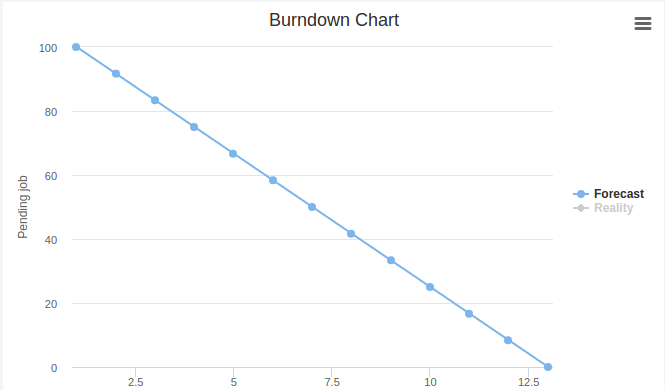
\includegraphics[scale=0.4]{img/graphics/burndown.png}
  \centering
  \caption{Burdown estimation chart.}
\end{figure}

\noindent Now is where play the mechanism Sprint Planning, Daily Scrum and the Sprint
Review Meeting. For each sprint of this thirteen, we must do a sprint planning
to know what issues are inside and which would put in the backlog and another
meeting to review the evolution of sprint.Normally another meeting must be done
diary, but in this case with the form of the team is not possible, so instead of is important, is not at the rest.
